\chapter{Especificación de Requisitos}

A especificación de requisitos segue a estrutura do estándar \textbf{IEEE~830}~\cite{ieee830} para
documentos de especificación de requisitos software (SRS), adaptada ás necesidades
deste proxecto: unha descrición xeral do produto, as interfaces con outros sistemas, os
requisitos funcionais e non funcionais, os casos de uso máis relevantes e a información
que o sistema debe almacenar.

\section{Descrición xeral}

\subsection{Perspectiva do produto}

Telaria é unha aplicación móbil baseada nunha arquitectura cliente–servidor. O frontend,
desenvolvido con React Native e Expo, comunícase cun backend Spring Boot mediante unha
API REST documentada con OpenAPI. O backend integra á súa vez servizos externos: un
motor de inferencia de linguaxe (Ollama) para o asistente de IA e un almacén de obxectos
compatible con S3 para os documentos compartidos.

\subsection{Funcionalidade do produto}

O sistema está composto polos seguintes módulos funcionais:

\begin{itemize}
  \item Autenticación e xestión de conta de usuario.
  \item Creación e adhesión a viaxes, xestión de membros.
  \item Rexistro de gastos compartidos e cálculo de liquidacións.
  \item Planificación de eventos con localización xeográfica.
  \item Almacenamento de documentos compartidos.
  \item Chat de grupo entre membros da viaxe.
  \item Asistente conversacional de intelixencia artificial por viaxe.
  \item Rede de amizades entre usuarios.
\end{itemize}

\subsection{Características dos usuarios}

\begin{tabularx}{\textwidth}{@{}lX@{}}
  \toprule
  \textbf{Tipo} & \textbf{Descrición} \\
  \midrule
  Usuario & Persoa rexistrada na aplicación. Pode crear ou unirse a viaxes e, dentro delas, ten acceso completo a todas as funcionalidades de forma colaborativa e en igualdade de condicións que o resto de membros. \\
  \bottomrule
\end{tabularx}

\subsection{Restricións}

\begin{itemize}
  \item A aplicación é multiplataforma (iOS e Android) e funciona sobre Expo.
  \item Toda comunicación co servidor realízase mediante HTTP e API REST.
  \item O sistema require conexión á rede para a totalidade das súas operacións.
\end{itemize}

\subsection{Suposicións e dependencias}

\begin{itemize}
  \item O servizo Ollama está dispoñible e accesible no servidor para o módulo de IA.
  \item A base de datos PostgreSQL está operativa e accesible para a persistencia de datos.
  \item Existe un servizo de almacenamento compatible co protocolo S3 para os documentos.
  \item Os requisitos aquí descritos son estables durante o desenvolvemento.
\end{itemize}

% -----------------------------------------------------------------------
\section{Interfaces con outros sistemas}

\subsection{Interface de usuario}

Interface gráfica móbil nativa (React Native) adaptada a iOS e Android sen necesidade
de compilación separada por plataforma.

\subsection{Interfaces de hardware}

\begin{itemize}
  \item Dispositivo móbil do usuario con sistema operativo iOS ou Android e conexión á rede.
  \item Servidor con capacidade para executar contedores Podman.
\end{itemize}

\subsection{Interfaces de software}

\begin{tabularx}{\textwidth}{@{}lX@{}}
  \toprule
  \textbf{Sistema} & \textbf{Descrición} \\
  \midrule
  API REST propia & Interface principal entre frontend e backend; documentada con OpenAPI/Swagger e consumida mediante JSON sobre HTTP. \\
  Ollama          & Servizo local de inferencia de modelos de linguaxe grande, accedido por HTTP para alimentar o asistente conversacional. \\
  Almacenamento S3 & Servizo de almacenamento de obxectos (compatible con S3) para a subida e descarga de documentos compartidos. \\
  PostgreSQL       & Base de datos relacional para a persistencia de todas as entidades do sistema. \\
  \bottomrule
\end{tabularx}

\subsection{Interfaces de comunicación}

O frontend e o backend comunícanse mediante HTTP. A autenticación baséase en dous
tokens: un \textit{access token} JWT de vida curta incluído en cada petición, e un
\textit{refresh token} opaco de vida longa almacenado no servidor e utilizado para
renovar o \textit{access token} sen necesidade de volver a autenticarse.

% -----------------------------------------------------------------------
\section{Requisitos funcionais}

\begin{longtable}{@{}p{1.2cm}p{3cm}p{8.5cm}p{1.5cm}@{}}
  \toprule
  \textbf{ID} & \textbf{Nome} & \textbf{Descrición} & \textbf{Prior.} \\
  \midrule
  \endfirsthead
  \toprule
  \textbf{ID} & \textbf{Nome} & \textbf{Descrición} & \textbf{Prior.} \\
  \midrule
  \endhead
  % -- Autenticación e conta --
  RF01 & Rexistro de usuario        & O sistema permite crear unha conta con nome de usuario, correo electrónico e contrasinal.                                                                                        & Alta   \\[4pt]
  RF02 & Autenticación              & O sistema autentica usuarios mediante un \textit{access token} JWT; o \textit{refresh token} opaco invalídase no peche de sesión.                                                  & Alta   \\[4pt]
  RF03 & Xestión do perfil          & Un usuario pode consultar e actualizar o seu nome de usuario e correo electrónico (o cambio de correo require a confirmación do contrasinal), cambiar o contrasinal e subir ou consultar o seu avatar. & Media  \\[4pt]
  RF04 & Eliminación de conta       & Un usuario pode eliminar a súa propia conta; a operación require a confirmación do contrasinal e elimina os datos persoais asociados.                                               & Baixa  \\[4pt]
  RF05 & Preferencias da aplicación & O usuario pode personalizar a interface: seleccionar o tema visual (claro ou escuro), o idioma (galego, castelán ou inglés) e activar o modo de aforro de datos.                    & Baixa  \\[4pt]
  % -- Viaxes e membros --
  RF06 & Crear viaxe                & Un usuario autenticado pode crear novas viaxes.                                                                                                                                     & Alta   \\[4pt]
  RF07 & Unirse a viaxe             & Un usuario pode unirse a unha viaxe mediante invitación recibida, solicitude de unión ou código QR.                                                                                 & Alta   \\[4pt]
  RF08 & Xestión de membros         & Calquera membro pode invitar outros usuarios á viaxe e xestionar as solicitudes de unión pendentes.                                                                                 & Alta   \\[4pt]
  RF09 & Saír dunha viaxe           & Calquera membro pode abandonar unha viaxe; se é o último membro, a viaxe e todos os seus datos asociados elimínanse automaticamente.                                                & Media  \\[4pt]
  % -- Gastos --
  RF10 & Xestión de gastos          & Calquera membro pode rexistrar un gasto (importe, nome, categoría, usuario pagador e conxunto de beneficiarios), ver os gastos da viaxe, ver os detalles dun gasto ou eliminalo.            & Alta   \\[4pt]
  RF11 & Liquidacións               & O sistema calcula automaticamente as liquidacións entre membros, minimizando o número de transferencias necesarias para saldar as débedas; ademais, calquera membro pode rexistrar liquidacións xa realizadas e consultar o histórico de liquidacións da viaxe. & Alta   \\[4pt]
  % -- Eventos --
  RF12 & Xestión de eventos         & Calquera membro pode crear, consultar e eliminar eventos con nome, data e hora de inicio, duración e localización xeográfica (nome, enderezo e coordenadas xeográficas).          & Alta  \\[4pt]
  % -- Documentos --
  RF13 & Documentos compartidos     & Calquera membro pode subir, consultar e eliminar documentos asociados á viaxe; os documentos de imaxe mostran unha miniatura de previsualización xerada automaticamente.                                                                                                   & Alta   \\[4pt]
  % -- Comunicación --
  RF14 & Chat de grupo              & Os membros dunha viaxe poden enviar e consultar mensaxes de texto no chat común da viaxe.                                                                                           & Media  \\[4pt]
  RF15 & Asistente de IA            & Cada viaxe dispón dun chatbot conversacional con historial persistente entre sesións.                                                                                               & Baixa  \\[4pt]
  % -- Amizades --
  RF16 & Rede de amizades           & Un usuario pode enviar solicitudes de amizade a outro (polo seu identificador ou código QR), aceptalas ou rexeitalas, consultar a súa lista de amigos e eliminar amizades.   & Baixa  \\[4pt]
  RF17 & Convidar amigos á viaxe    & Permite convidar amigos a unha viaxe directamente dende a lista de amizades, como atallo ás invitacións por identificador ou QR.                  & Baixa  \\
  \bottomrule
\end{longtable}

% -----------------------------------------------------------------------
\section{Casos de uso}

A partir dos requisitos funcionais identifícanse os casos de uso máis relevantes do
sistema. Dado que non existe distinción de roles, o único actor é o \textbf{Usuario}
rexistrado, que interactúa con todas as funcionalidades. A
Figura~\ref{fig:casos-uso} resume os casos de uso agrupados por área funcional, e a
continuación detállanse os fluxos principais.

\begin{figure}[H]
  \centering
  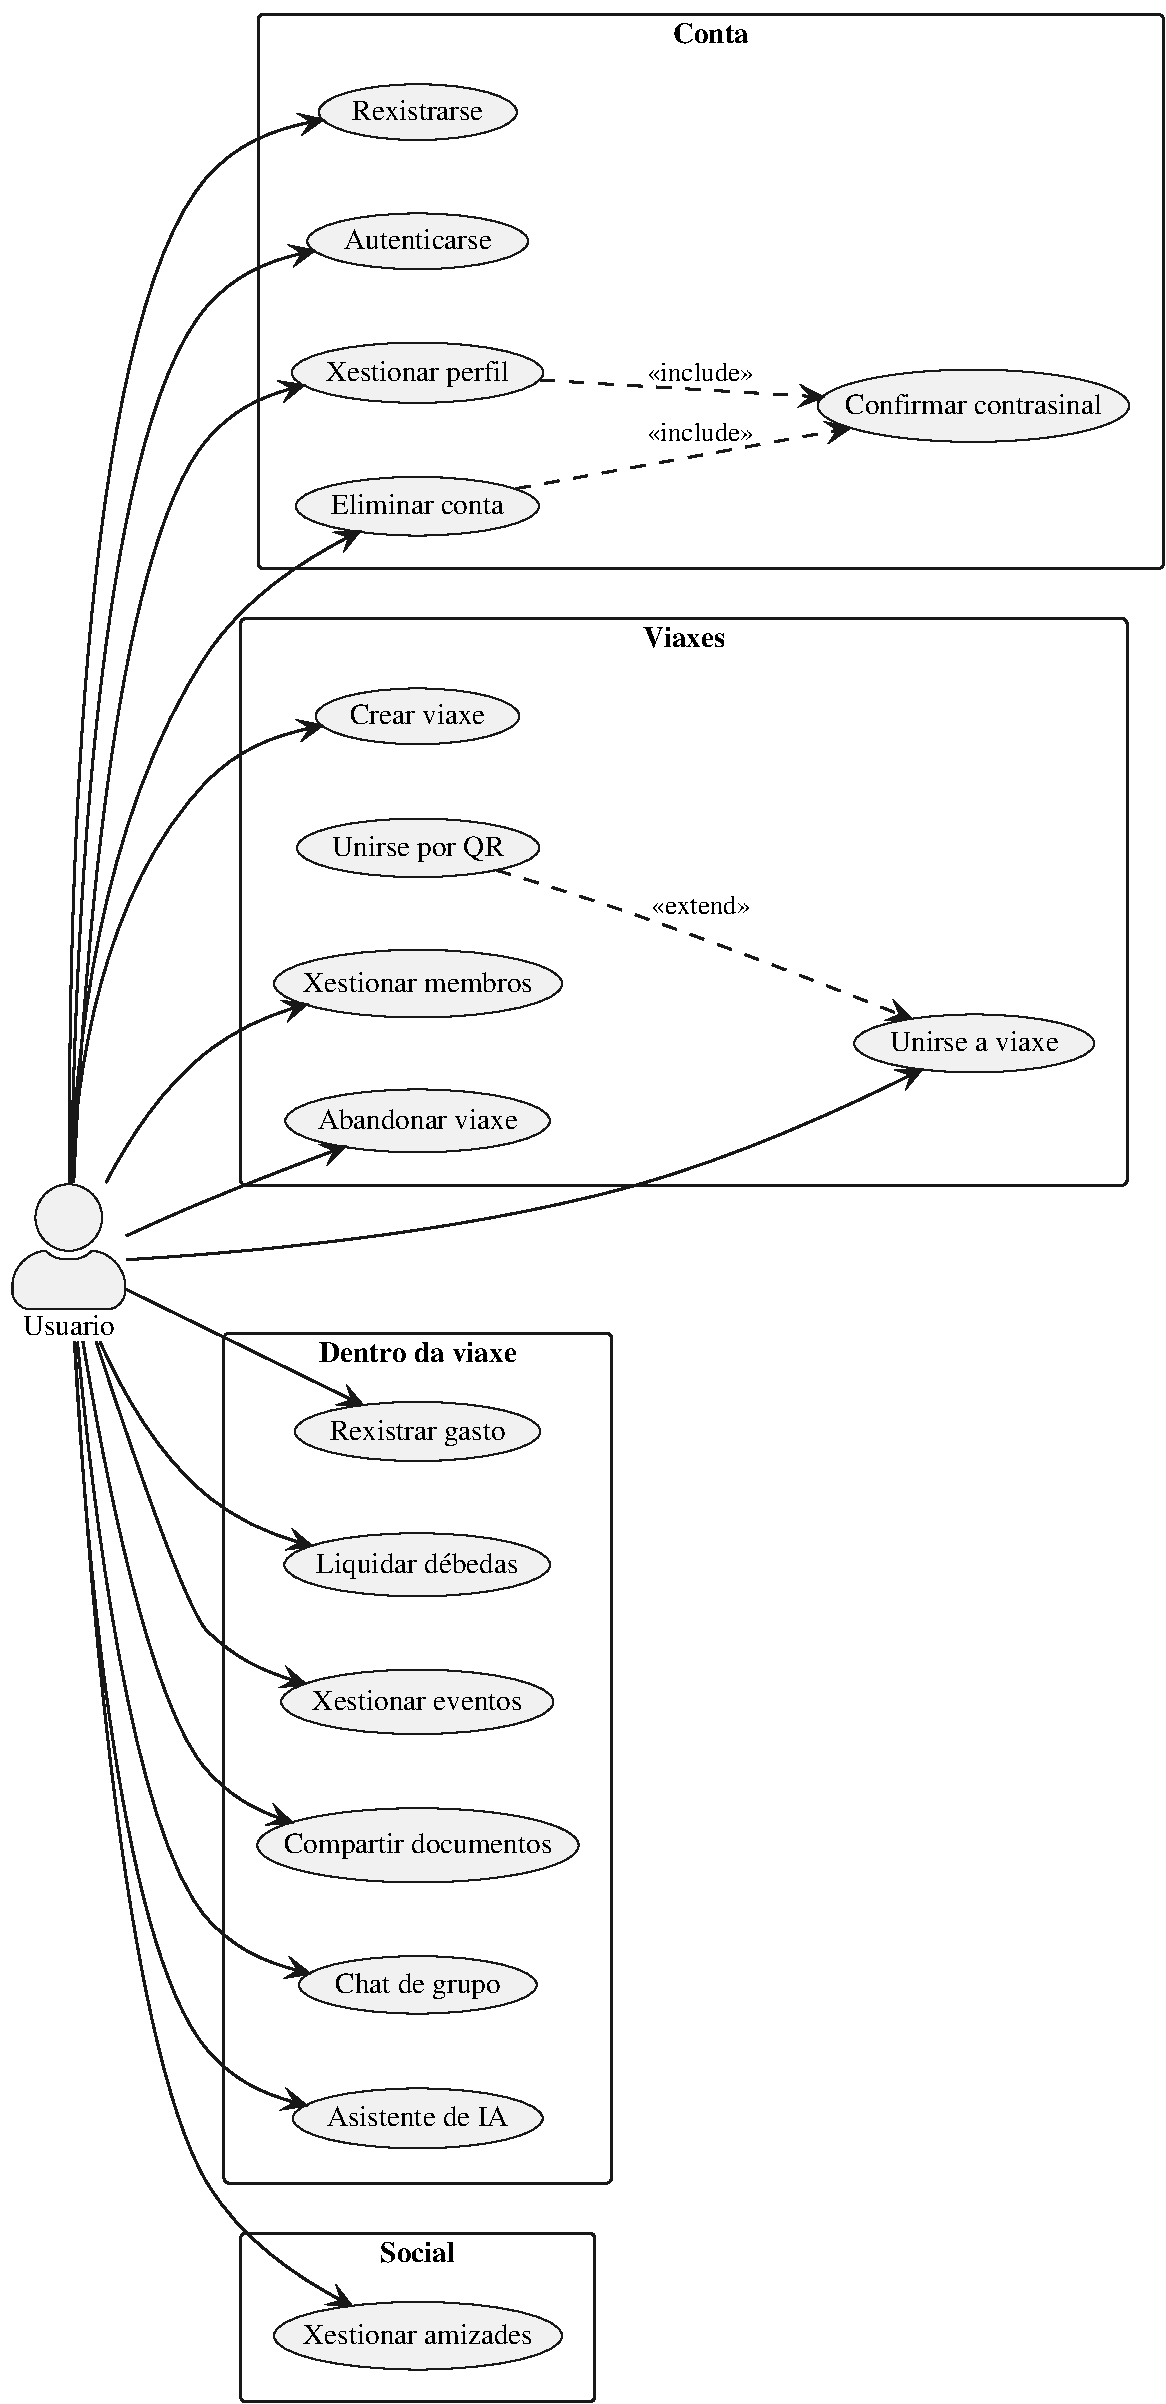
\includegraphics[width=0.52\textwidth]{diagrams/casos-uso.pdf}
  \caption{Diagrama de casos de uso de Telaria (actor único: Usuario).}
  \label{fig:casos-uso}
\end{figure}

\paragraph*{CU01. Rexistro e autenticación.}
\begin{itemize}[noitemsep,topsep=2pt]
  \item \textbf{Actor:} Usuario.
  \item \textbf{Precondicións:} dispón da aplicación instalada e de conexión á rede.
  \item \textbf{Fluxo principal:} (1) introduce nome de usuario, correo e contrasinal e solicita o rexistro; (2) o sistema crea a conta, almacena o contrasinal cifrado e devolve un \textit{access token} JWT e un \textit{refresh token}; (3) o usuario queda autenticado. O inicio de sesión posterior realízase con correo e contrasinal.
  \item \textbf{Fluxos alternativos:} correo xa rexistrado $\rightarrow$ o sistema rexeita o rexistro; credenciais incorrectas no inicio de sesión $\rightarrow$ erro de autenticación; caducidade do \textit{access token} $\rightarrow$ o cliente renóvao de forma transparente co \textit{refresh token}.
  \item \textbf{Poscondición:} o usuario dispón dunha sesión activa.
  \item \textbf{Requisitos:} RF01, RF02.
\end{itemize}

\paragraph*{CU02. Unirse a unha viaxe.}
\begin{itemize}[noitemsep,topsep=2pt]
  \item \textbf{Actor:} Usuario.
  \item \textbf{Precondicións:} usuario autenticado.
  \item \textbf{Fluxo principal (por invitación):} (1) un membro da viaxe convída ao usuario; (2) o usuario recibe a notificación e acepta a invitación; (3) o sistema rexistra a adhesión e o usuario pasa a ser membro da viaxe.
  \item \textbf{Fluxos alternativos:} por solicitude (o usuario solicita unirse a partir dun identificador de viaxe e calquera membro aproba a solicitude); por QR (o usuario escanea un código QR que o sistema procesa como invitación directa).
  \item \textbf{Poscondición:} o usuario figura na lista de membros da viaxe.
  \item \textbf{Requisitos:} RF07, RF08.
\end{itemize}

\paragraph*{CU03. Rexistrar un gasto e liquidar débedas.}
\begin{itemize}[noitemsep,topsep=2pt]
  \item \textbf{Actor:} Usuario (membro da viaxe).
  \item \textbf{Precondicións:} o usuario é membro da viaxe.
  \item \textbf{Fluxo principal:} (1) rexistra un gasto (importe, nome, categoría, pagador e beneficiarios); (2) o sistema garda o gasto e recalcula os balances; (3) o membro consulta quen debe a quen; (4) cando se salda unha débeda, rexístrase a liquidación correspondente.
  \item \textbf{Fluxos alternativos:} o pagador ou algún beneficiario non é membro da viaxe $\rightarrow$ erro de validación.
  \item \textbf{Poscondición:} os balances reflicten o novo gasto; as liquidacións rexistradas reducen as débedas pendentes.
  \item \textbf{Requisitos:} RF10, RF11.
\end{itemize}

\paragraph*{CU04. Xestionar os membros da viaxe.}
\begin{itemize}[noitemsep,topsep=2pt]
  \item \textbf{Actor:} Usuario (membro da viaxe).
  \item \textbf{Precondicións:} o usuario é membro da viaxe.
  \item \textbf{Fluxo principal:} (1) convida a outro usuario (por identificador, amizade ou QR) ou consulta as solicitudes de unión pendentes; (2) acepta ou rexeita unha solicitude; (3) o sistema actualiza a lista de membros.
  \item \textbf{Fluxos alternativos:} usuario xa membro ou xa convidado $\rightarrow$ conflito.
  \item \textbf{Poscondición:} a composición da viaxe queda actualizada. Calquera membro pode realizar estas accións: non hai roles.
  \item \textbf{Requisitos:} RF08, RF17.
\end{itemize}

\paragraph*{CU05. Subir un documento.}
\begin{itemize}[noitemsep,topsep=2pt]
  \item \textbf{Actor:} Usuario (membro da viaxe).
  \item \textbf{Precondicións:} o usuario é membro da viaxe.
  \item \textbf{Fluxo principal:} (1) inicia a subida indicando nome e tipo de contido; (2) o sistema crea o rexistro e devolve unha URL prefirmada; (3) o cliente sobe o ficheiro directamente ao almacén de obxectos; (4) o cliente confirma a subida e o sistema marca o documento como dispoñible, xerando unha miniatura de forma asíncrona se é unha imaxe.
  \item \textbf{Fluxos alternativos:} se a subida non se confirma, unha tarefa programada verifica a existencia do arquivo no almacenamento e, de existir, a marca como confirmada; en caso contrario, elimina o rexistro orfo.
  \item \textbf{Poscondición:} o documento queda listado e descargable mediante URL prefirmada.
  \item \textbf{Requisitos:} RF13.
\end{itemize}

\paragraph*{CU06. Eliminar a conta.}
\begin{itemize}[noitemsep,topsep=2pt]
  \item \textbf{Actor:} Usuario.
  \item \textbf{Precondicións:} usuario autenticado.
  \item \textbf{Fluxo principal:} (1) solicita eliminar a súa conta; (2) o sistema solicita a confirmación do contrasinal; (3) tras a verificación, elimínanse os datos persoais e os artefactos asociados (avatares, documentos) e retírase o usuario das viaxes compartidas; (4) péchase a sesión.
  \item \textbf{Fluxos alternativos:} contrasinal incorrecto $\rightarrow$ cancélase a operación.
  \item \textbf{Poscondición:} a conta e os datos persoais quedan eliminados.
  \item \textbf{Requisitos:} RF03, RF04.
\end{itemize}

% -----------------------------------------------------------------------
\section{Requisitos non funcionais}

\subsection{Seguridade}

\begin{itemize}
  \item \textbf{RNF-SE-01}. Control de acceso: só os membros dunha viaxe acceden aos seus datos; calquera usuario autenticado pode crear viaxes.
  \item \textbf{RNF-SE-02}. Os contrasinais almacénanse con hash BCrypt; os \textit{access tokens} JWT teñen vida curta e os \textit{refresh tokens} opacos almacénanse no servidor para limitar a exposición ante intrusións.
  \item \textbf{RNF-SE-03}. As operacións sensibles sobre a conta (o cambio de correo electrónico e a eliminación da conta) requiren a confirmación do contrasinal actual.
\end{itemize}

\subsection{Privacidade e protección de datos}

\begin{itemize}
  \item \textbf{RNF-PR-01}. A eliminación da conta borra os datos persoais do usuario e os artefactos asociados no almacén de obxectos (avatar e documentos), e retírao das viaxes compartidas.
  \item \textbf{RNF-PR-02}. As mensaxes de chat (de grupo e do asistente de IA) elimínanse automaticamente tras un período de retención de 30 días mediante unha tarefa programada.
\end{itemize}

\subsection{Rendemento}

\begin{itemize}
  \item \textbf{RNF-RE-01}. O cálculo de liquidacións realízase no servidor, evitando sobrecargar o dispositivo cliente.
  \item \textbf{RNF-RE-02}. A entrega de mensaxes do chat e das respostas do asistente de IA realízase en tempo real mediante eventos enviados polo servidor (SSE).
  \item \textbf{RNF-RE-03}. A xeración de miniaturas dos documentos de imaxe execútase de forma asíncrona, fóra da ruta de petición, para non penalizar a latencia da subida nin da listaxe.
\end{itemize}

\subsection{Usabilidade}

\begin{itemize}
  \item \textbf{RNF-US-01}. A interface debe ser intuitiva e usable sen formación previa.
  \item \textbf{RNF-US-02}. A aplicación estará dispoñible en galego, castelán e inglés.
  \item \textbf{RNF-US-03}. A aplicación proporcionará retroalimentación visual inmediata
        ante cada acción relevante (indicadores de carga, confirmacións e mensaxes de erro),
        conforme ao heurístico de visibilidade do estado do sistema de Nielsen.
  \item \textbf{RNF-US-04}. A interface será consistente en terminoloxía, iconas e
        comportamento en todas as pantallas, seguindo o heurístico de coherencia e estándares
        de Nielsen.
  \item \textbf{RNF-US-05}. A paleta de cores respectará os estándares de accesibilidade:
        a información crítica non dependerá unicamente da cor, de xeito que sexa interpretable
        por usuarios con déficit de percepción cromática.
\end{itemize}

\subsection{Mantibilidade}

\begin{itemize}
  \item \textbf{RNF-MA-01}. O contrato OpenAPI é a fonte de verdade da API: a partir del xéranse automaticamente as interfaces e DTO do backend e os tipos do frontend, garantindo a sincronía entre ambos os extremos.
  \item \textbf{RNF-MA-02}. A lóxica do backend está cuberta por unha batería de probas automatizadas (unitarias e de integración) que facilita a evolución segura do código.
\end{itemize}

\subsection{Portabilidade e despregamento}

\begin{itemize}
  \item \textbf{RNF-PO-01}. O backend e os servizos auxiliares despreganse en contedores Podman.
  \item \textbf{RNF-PO-02}. A aplicación móbil é compatible con iOS e Android mediante Expo/React Native.
\end{itemize}

\subsection{Interoperabilidade}

\begin{itemize}
  \item \textbf{RNF-IN-01}. O almacenamento de documentos baséase no protocolo estándar S3, o que garante a independencia respecto dun provedor concreto.
\end{itemize}

\subsection{Fiabilidade}

\begin{itemize}
  \item \textbf{RNF-FI-01}. O sistema valida os datos de entrada na API e devolve mensaxes de erro claras e estruturadas ao cliente.
  \item \textbf{RNF-FI-02}. Unha tarefa programada reconcilia periodicamente as subidas de documentos non confirmadas (orfas): confirma as que efectivamente existen no almacén de obxectos e elimina os rexistros sen ficheiro asociado, evitando entradas inconsistentes na base de datos.
\end{itemize}

% -----------------------------------------------------------------------
\section{Información que o sistema debe almacenar}

A persistencia do sistema repártese en tres niveis complementarios segundo a natureza do
dato. A información estruturada do dominio (usuarios, viaxes, eventos, gastos, mensaxes,
etc.) almacénase nunha base de datos relacional \textbf{PostgreSQL}, onde Hibernate mapea
cada entidade á súa táboa. Os \textbf{ficheiros binarios} (documentos compartidos e
avatares) non se gardan na base de datos, senón nun \textbf{almacén de obxectos}. Por
último, o dispositivo do usuario conserva localmente un pequeno conxunto de datos de
sesión e de preferencias que se detalla máis adiante. O Cadro~\ref{tab:entidades} recolle
as principais entidades persistidas no servidor e os seus atributos.

\begin{longtable}{@{}p{4cm}p{10.3cm}@{}}
  \caption{Entidades persistidas no servidor.}
  \label{tab:entidades} \\
  \toprule
  \textbf{Entidade} & \textbf{Atributos principais} \\
  \midrule
  \endfirsthead
  \caption*{Cadro~\ref{tab:entidades} (continuación)} \\
  \toprule
  \textbf{Entidade} & \textbf{Atributos principais} \\
  \midrule
  \endhead
  Usuario                    & Identificador (UUID), nome de usuario, correo electrónico, contrasinal (hash). \\[4pt]
  Viaxe                      & Identificador (UUID), nome, data de creación, conxunto de membros (usuarios). \\[4pt]
  Evento                     & Identificador, nome, data e hora de inicio (con fuso horario), duración en minutos, localización embebida (nome, enderezo, latitude, lonxitude). \\[4pt]
  Gasto                      & Identificador, importe (decimal), nome, categoría (enumeración), usuario pagador, usuario creador do rexistro, conxunto de beneficiarios, marca temporal. \\[4pt]
  Liquidación                & Identificador, importe (decimal), usuario pagador, usuario receptor, marca temporal. \\[4pt]
  Documento compartido       & Identificador, nome de ficheiro, clave no almacén de obxectos, clave da miniatura de previsualización, estado de subida (booleano), usuario creador, marca temporal. \\[4pt]
  Invitación / Solicitude    & Identificador, usuario, viaxe asociada, marca temporal de creación. \\[4pt]
  Amizade                    & Identificador (UUID), dous usuarios asociados (almacenados de forma normalizada para garantir a unicidade da parella), marca temporal de creación. \\[4pt]
  Solicitude de amizade      & Identificador (UUID), usuario emisor, usuario receptor, marca temporal de creación. \\[4pt]
  Mensaxe de chat de grupo   & Identificador, contido (texto), autor, viaxe asociada, marca temporal. \\[4pt]
  Mensaxe de asistente de IA & Identificador, contido (texto), rol (USUARIO ou ASISTENTE), usuario, viaxe asociada, marca temporal. \\[4pt]
  Token de refresco          & Token (identificador), identificador do usuario asociado. \\
  \bottomrule
\end{longtable}

\subsection{Almacenamento de ficheiros (MinIO)}

Os ficheiros que sobe o usuario (documentos compartidos das viaxes e imaxes de avatar)
non son axeitados para gardarse nunha base de datos relacional: trátase de obxectos
binarios potencialmente grandes que cargarían as táboas, dificultarían as copias de
seguranza e penalizarían o rendemento das consultas. Por iso o sistema delega a súa
custodia nun \textbf{almacén de obxectos compatible coa API de Amazon~S3}, para o que se
emprega \textbf{MinIO}, unha solución de código aberto. A vantaxe de MinIO é que é
\textbf{autoxestionado}: en lugar de contratar un servizo de almacenamento na nube como
Amazon~S3 (onde os ficheiros residen na infraestrutura dun provedor externo e o seu uso se
factura por consumo), MinIO execútase na propia infraestrutura do proxecto, despregándose
de xeito sinxelo como un contedor (Docker / Podman) xunto co resto de servizos. Isto
elimina a dependencia e os custos dun provedor comercial e, ao expoñer a mesma API que
S3, permitiría migrar a ese servizo no futuro sen apenas cambios no código.

A base de datos non garda o contido do ficheiro, senón unicamente os \textbf{metadatos}
necesarios para localizalo: a clave do obxecto dentro do almacén (\textit{object key}), a
clave da miniatura de previsualización e o estado da subida. Deste xeito mantense unha
única fonte de verdade (o rexistro relacional referencia o obxecto físico) e evítase a
duplicación de datos pesados.

A interacción co almacén realízase mediante \textbf{URLs prefirmadas}: cando un usuario
quere subir ou descargar un ficheiro, o backend xera unha URL temporal e asinada que
autoriza esa operación concreta durante un período limitado. O cliente comunícase
\textbf{directamente} con MinIO empregando esa URL, polo que o servidor de aplicación
nunca chega a recibir nin a servir os bytes do ficheiro. Esta arquitectura descarga o
backend, mellora a escalabilidade e reduce a latencia das transferencias.

\subsection{Información almacenada no dispositivo (frontend)}

Ademais da persistencia no servidor, a aplicación móbil garda localmente no dispositivo un
conxunto reducido de información para soster a sesión entre execucións e recordar as
preferencias da persoa usuaria. As credenciais de sesión (os \textit{tokens}) gárdanse no
\textbf{almacén seguro e cifrado do sistema operativo}, respaldado pola \textit{keychain}
de iOS ou o \textit{keystore} de Android, mentres que o resto de valores, ao non ser
sensibles, se persisten no almacenamento clave-valor convencional do dispositivo. O
Cadro~\ref{tab:frontend-storage} resume o que se garda no cliente.

\begin{longtable}{@{}p{3.6cm}p{10.7cm}@{}}
  \caption{Datos persistidos localmente no dispositivo do cliente.}
  \label{tab:frontend-storage} \\
  \toprule
  \textbf{Clave} & \textbf{Contido e propósito} \\
  \midrule
  \endfirsthead
  \toprule
  \textbf{Clave} & \textbf{Contido e propósito} \\
  \midrule
  \endhead
  \texttt{refreshToken} & Token de refresco da sesión (cifrado); permite obter novos tokens de acceso sen volver iniciar sesión. \\[3pt]
  \texttt{accessToken}  & Token de acceso vixente (cifrado) que autoriza as peticións á API. \\[3pt]
  \texttt{userEmail}    & Correo electrónico da persoa usuaria autenticada. \\[3pt]
  \texttt{username}     & Nome de usuario mostrado na interface. \\[3pt]
  \texttt{app\_language} & Idioma escollido para a interface (es / en / gl). \\[3pt]
  \texttt{app\_theme}    & Tema visual seleccionado (claro / escuro). \\[3pt]
  \texttt{app\_data\_saver} & Indicador do modo de aforro de datos. \\[3pt]
  \texttt{lastTripId}   & Identificador da última viaxe aberta, para restaurar a navegación. \\[3pt]
  \texttt{lastTripTab}  & Última pestana visitada dentro dunha viaxe. \\
  \bottomrule
\end{longtable}

Este almacenamento local é deliberadamente mínimo: non se replica no dispositivo o
contido das viaxes nin datos doutros usuarios, senón unicamente o estritamente preciso
para reanudar a sesión e personalizar a experiencia. Ao pechar sesión, tanto as
credenciais cifradas como o estado de navegación bórranse do dispositivo.
